%!TEX root = ../pres.tex
\begin{frame}
\frametitle{Q-Learning}
  \begin{center}\textbf{Goals of Q-learning}\end{center}
  \begin{enumerate}
    \onslide<1->{\item Approximate $Q^{\pi^*}$, the $Q$ function of the optimal agent, as $Q(s_t, a_t)$.}
    \onslide<2->{\item Using $Q$, find the agent, $\pi$, that best approximates the optimal agent, $\pi^*$.}
  \end{enumerate}
\end{frame}

\begin{frame}
\frametitle{Q-Learning}
  \onslide<1->{\begin{center}\textbf{How do we define best?}\end{center}}
  \onslide<2->{
  Given some state $s_t$, the \textbf{best} agent, $\pi^*$ is one that takes action 
    \begin{equation*}
      a_t = \arg \max_a Q(s_t, a).   
    \end{equation*}
  }
\end{frame}

\begin{frame}
\frametitle{Q-Learning}
  \begin{center}
  \textbf{An example: Frozen Lake Problem}
  \includegraphics[width=0.5\textwidth]{frozen-lake.png}
  \end{center}

\end{frame}
\begin{frame}
\frametitle{Q-Learning}
  \begin{columns}
    \begin{column}{0.5\textwidth}
    \begin{itemize}
      \item $100$ reward for reaching the goal
      \item $0$ otherwise
    \end{itemize}
    \onslide<1->{\textbf{How do we keep track of this long term reward?}}
    \onslide<2->{\begin{center}\textbf{$Q$ function}\end{center}}
    \end{column}
    \begin{column}{0.5\textwidth}
      \includegraphics[width=0.9\textwidth]{frozen-lake.png}
    \end{column}
  \end{columns}
\end{frame}
\begin{frame}
\frametitle{Q-Learning}
  \begin{center}
    \textbf{How do we actually calculate the $Q$ function?}
  \end{center}
  \onslide<2->{
  \begin{center}
  \textbf{The Bellman Equation.}
  }
  \onslide<3->{
  \begin{equation*}
      Q^\pi(s_t, a_t) = r_t + \gamma Q^\pi(s_{t+1}, \pi(s_{t+1}))
  \end{equation*}
  \end{center}
}
\end{frame}

\begin{frame}
\frametitle{Q-Learning}
  \textbf{One $Q$-Learning Algorithm: Tabular Q-Learning}
  \begin{itemize}
    \item Explore the environment
    \item On the way, use the Bellman equation to store a table of expected future reward ($Q$) for each state-action pair.
    \item Use this table to pick the best possible action for any given state.
  \end{itemize}
\end{frame}

\begin{frame}
\frametitle{Q-Learning}
  \begin{columns}
    \begin{column}{0.5\textwidth}
  \textbf{An example update for Frozen Lake.}
  
  Suppose our stored $Q$ table looks like so:
  \begin{center}\scalebox{0.5}{\begin{tabular}{ | c | c | c | c |}
    \multicolumn{1}{c}{Up} &\multicolumn{1}{c}{Down} & \multicolumn{1}{c}{Left} & \multicolumn{1}{c}{Right} \\\hline
    0 & 65 & 0 & 40 \\
    0 & 0 & 0 & 0 \\
    0 & 0 & 0 & 0 \\
    0 & 0 & 0 & 0 \\
    50 & 75 & 30 & 20 \\
    0 & 0 & 0 & 0 \\
    0 & 0 & 0 & 0 \\
    0 & 0 & 0 & 0 \\
    0 & 0 & 0 & 0 \\
    0 & 0 & 0 & 0 \\
    0 & 0 & 0 & 0 \\
    0 & 0 & 0 & 0 \\
    0 & 0 & 0 & 0 \\
    0 & 0 & 0 & 0 \\
    0 & 0 & 0 & 0 \\
    0 & 0 & 0 & 0 \\\hline
  \end{tabular}   
  }\end{center}
    \end{column}
    \begin{column}{0.5\textwidth}
      \includegraphics[width=0.9\textwidth]{frozen-lake.png}
    \end{column}
  \end{columns}
\end{frame}

\begin{frame}
\frametitle{Q-Learning}
  \begin{columns}
    \begin{column}{0.5\textwidth}
  \textbf{An example update for Frozen Lake.} 
  
    Then suppose our agent moves \textbf{down} from the starting square
    \end{column}
    \begin{column}{0.5\textwidth}
      \includegraphics[width=0.9\textwidth]{frozen-lake-arrow.png}
    \end{column}
  \end{columns}
\end{frame}

\begin{frame}
\frametitle{Q-Learning}
  \textbf{An example update for Frozen Lake.} 
  
   Then we update using the Bellman equation.
   \begin{equation*}
     Q(s_{t+1}, a_{t+1}) = Q(s_t, a_t) + \alpha (r_t + \gamma (\max_a Q(s_t, a) - Q(s_t, a_t)) 
   \end{equation*}
    \begin{center}\scalebox{0.5}{\begin{tabular}{ | c | c | c | c |}
    \multicolumn{1}{c}{Up} &\multicolumn{1}{c}{Down} & \multicolumn{1}{c}{Left} & \multicolumn{1}{c}{Right} \\\hline
    0 & \cellcolor{yellow}65 & 0 & 40 \\
    0 & 0 & 0 & 0 \\
    0 & 0 & 0 & 0 \\
    0 & 0 & 0 & 0 \\
    \rowcolor{green}50 & 75 & 30 & 20 \\
    0 & 0 & 0 & 0 \\
    0 & 0 & 0 & 0 \\
    0 & 0 & 0 & 0 \\
    0 & 0 & 0 & 0 \\
    0 & 0 & 0 & 0 \\
    0 & 0 & 0 & 0 \\
    0 & 0 & 0 & 0 \\
    0 & 0 & 0 & 0 \\
    0 & 0 & 0 & 0 \\
    0 & 0 & 0 & 0 \\
    0 & 0 & 0 & 0 \\\hline
  \end{tabular}   
  }\end{center}
\end{frame}

\begin{frame}
\frametitle{Q-Learning}
  \textbf{An example update for Frozen Lake.} 

  The table now looks like so:
  \begin{center}\scalebox{0.5}{\begin{tabular}{ | c | c | c | c |}
    \multicolumn{1}{c}{Up} &\multicolumn{1}{c}{Down} & \multicolumn{1}{c}{Left} & \multicolumn{1}{c}{Right} \\\hline
    0 & 70 & 0 & 40 \\
    0 & 0 & 0 & 0 \\
    0 & 0 & 0 & 0 \\
    0 & 0 & 0 & 0 \\
    50 & 75 & 30 & 20 \\
    0 & 0 & 0 & 0 \\
    0 & 0 & 0 & 0 \\
    0 & 0 & 0 & 0 \\
    0 & 0 & 0 & 0 \\
    0 & 0 & 0 & 0 \\
    0 & 0 & 0 & 0 \\
    0 & 0 & 0 & 0 \\
    0 & 0 & 0 & 0 \\
    0 & 0 & 0 & 0 \\
    0 & 0 & 0 & 0 \\
    0 & 0 & 0 & 0 \\\hline
  \end{tabular}   
  }\end{center}
\end{frame}

\begin{frame}
\frametitle{Q-Learning}
  \textbf{Deep Q Learning}
    We can \emph{approximate} $Q$ with deep learning!
    \begin{enumerate}
      \item Make a neural network $\scriptn: \scripts \to \mathbb{R}^n$ which predicts 
      the future reward of taking each possible action
      \begin{equation*}
        \scriptn(s_t) =\begin{pmatrix}
            Q^*(s_t, a_1) \\
             Q^*(s_t, a_2)\\
             \vdots \\
              Q^*(s_t, a_n)
        \end{pmatrix}
      \end{equation*}
    \end{enumerate}
\end{frame}
\begin{frame}
\frametitle{Q-Learning}
  \textbf{Deep Q-Learning}
\begin{center}
  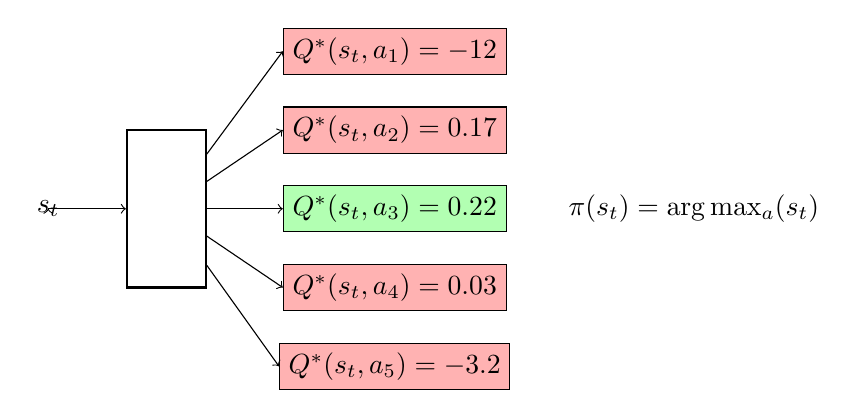
\begin{tikzpicture}
\node[rectangle] at (0,0) {$s_t$};
\node[rectangle] at (1.5,0) [draw,thick,minimum width=1cm,minimum height=2cm] (B) {$\scriptn$};
\node[rectangle] at (4.4, 2)  [draw, fill=red!30] (C1) {$Q^*(s_t,a_1) = -12$};
\node[rectangle] at (4.4, 1)  [draw, fill=red!30] (C2) {$Q^*(s_t,a_2) = 0.17$};
\node[rectangle] at (4.4, 0)  [draw, fill=green!30] (C3) {$Q^*(s_t,a_3) = 0.22$};
\node[rectangle] at (4.4, -1) [draw, fill=red!30]  (C4) {$Q^*(s_t,a_4) = 0.03$};
\node[rectangle] at (4.4, -2) [draw, fill=red!30]  (C5) {$Q^*(s_t,a_5) = -3.2$};
\node[rectangle] at (8.2, 0) (D) {$ \pi(s_t) =  \arg \max_a \scriptn(s_t)$};
\draw[->] (0,0) edge (B);
\draw[->] (B) edge (C1.west);
\draw[->] (B) edge (C2.west);
\draw[->] (B) edge (C3.west);
\draw[->] (B) edge (C4.west);
\draw[->] (B) edge (C5.west);
\end{tikzpicture} 
\end{center}
\end{frame}

